\section{Introduction}
%Deforestation in Amazon
{\setbeamertemplate{frame footer}{\href{https://earthobservatory.nasa.gov/world-of-change/Deforestation}{\textcolor{gray}{https://earthobservatory.nasa.gov/world-of-change/Deforestation}}}
	\begin{frame}{Deforestation in Amazon}
	\centering
	\animategraphics[loop,autoplay,width=\textwidth]{2}{amazon_deforestation-}{0}{12}
\end{frame}
}

%What is conservation biology?
{\setbeamertemplate{frame footer}{*\href{https://www.nature.com/subjects/conservation}{\textcolor{gray}{https://www.nature.com/subjects/conservation}}}
	\begin{frame}[t]{What is conservation biology?}
Conservation biology is the study of attempts to protect and preserve \alert{biodiversity}*.
\begin{block}<2->{It focuses on}
	\begin{itemize}		
		\item<2-> both the biological and social factors that affect the success of conservation efforts,
		\item<2-> determining ecosystems and species whose conservation is a high priority.
	\end{itemize}
\end{block}

\begin{block}<3->{It has two central goals}
	\begin{itemize}		
		\item<3-> to evaluate human impacts on biodiversity,
		\item<3-> to develop practical approaches to prevent the extinction of species \cite{wilson1992diversity} (Soulé 1986, Wilson 1992).
	\end{itemize}
\end{block}
\end{frame}}

%below will be a frame with only one picture full creeen:
%\begin{frame}[plain]
%\makebox[\linewidth]{\parbox{\paperwidth}{\animategraphics[loop,autoplay,width=\paperwidth]{5}{amazon_deforestation-}{0}{12}}}
%\end{frame}

%Why to preserve biodiversity?
{\setbeamertemplate{frame footer}{*\href{https://www.nature.com/scitable/knowledge/library/conservation-of-biodiversity-13235087}{\textcolor{gray}{https://www.nature.com/scitable/knowledge/library/conservation-of-biodiversity-13235087}}}
	\begin{frame}[t]{Why to preserve biodiversity?}
	\begin{itemize}
		\item Modern extinction rates are at \alert{100} to \alert{1000} times greater than background extinction rates calculated over the eras \cite{hambler2004extinction}.
		\item Existing species go extinct at a rate \alert{1000} times that of species formation*.
		\item The primary cause of today's loss of biodiversity is \alert{habitat alteration caused by human activities}.
	\end{itemize}	
\end{frame}
}

%Proportion of population using improved drinking water sources (\%), 1990
{\setbeamertemplate{frame footer}{\href{http://gamapserver.who.int/mapLibrary/Files/Maps/Global_water_1990.png}{\textcolor{gray}{http://gamapserver.who.int/mapLibrary/Files/Maps/Global\_water\_1990.png}}}
	\begin{frame}{Proportion of population using improved drinking water sources (\%), 1990}
	\makebox[\linewidth]{\parbox{\paperwidth}{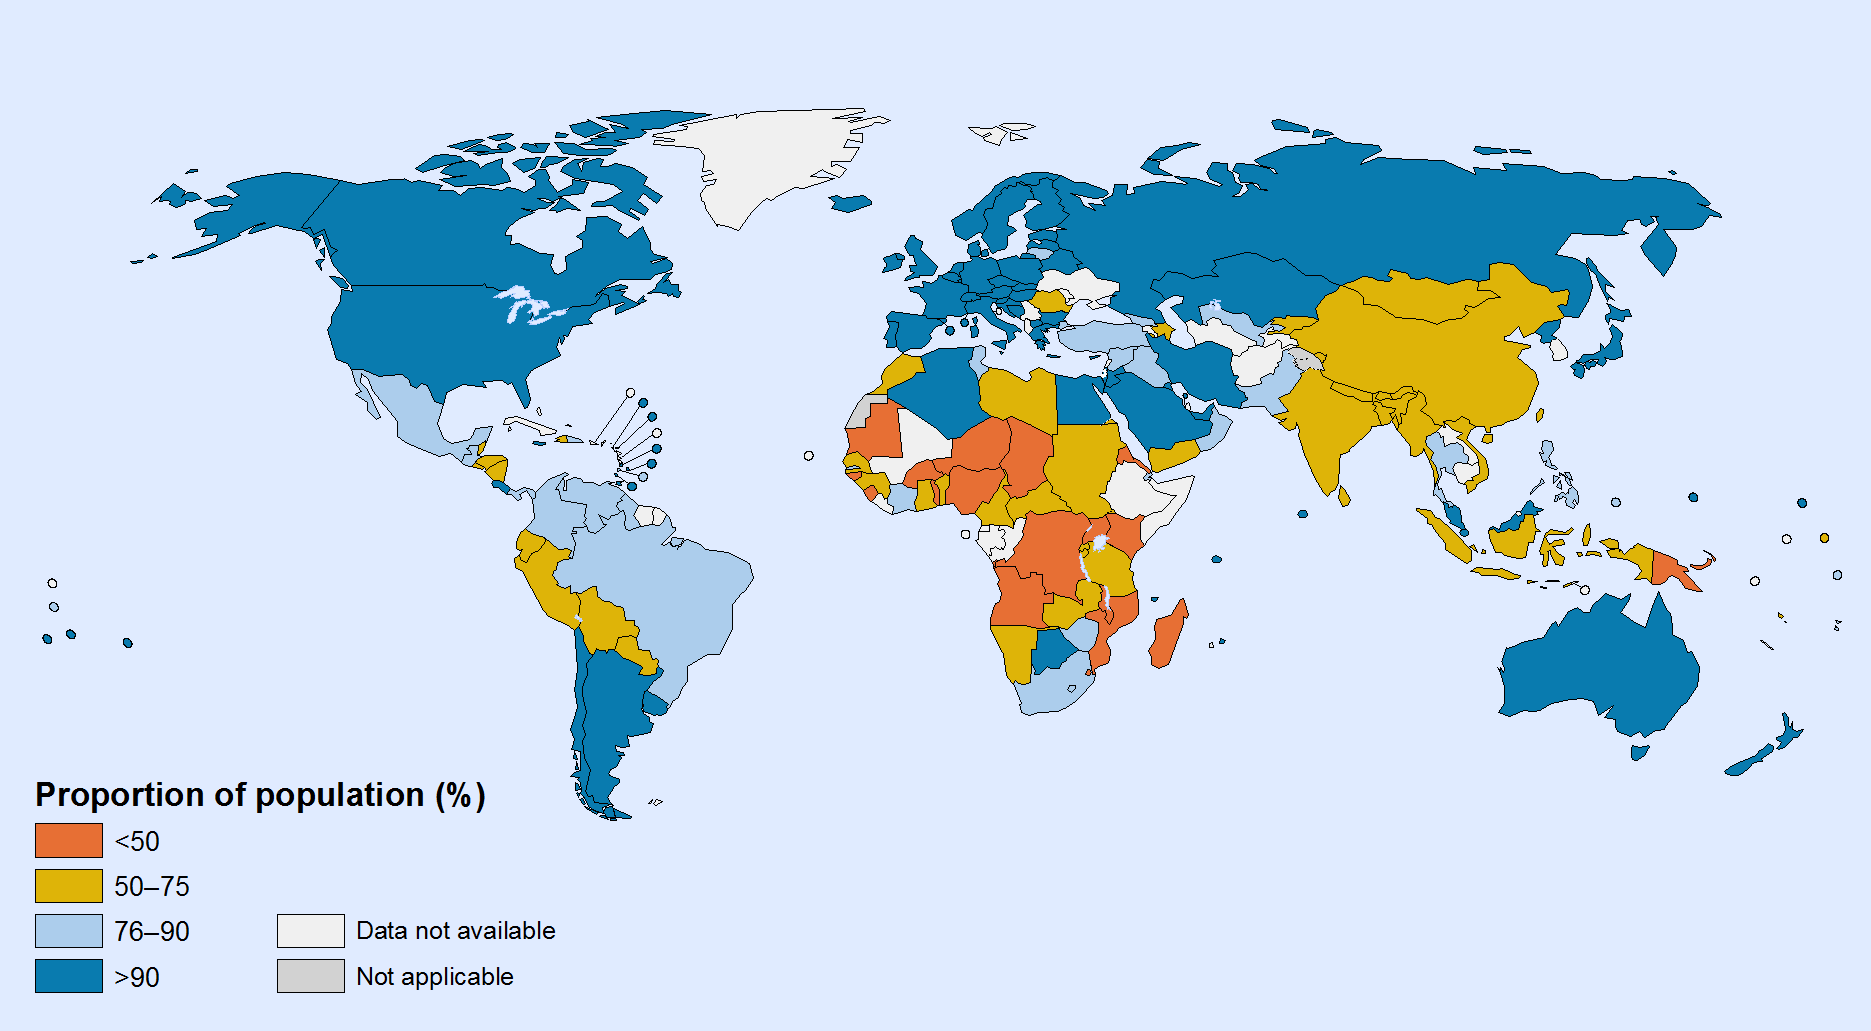
\includegraphics[width=\paperwidth]{Global_water_1990}}}
\end{frame}
}

%Proportion of population using improved sanitation facilities (\%), 1990
{\setbeamertemplate{frame footer}{\href{http://gamapserver.who.int/mapLibrary/Files/Maps/Global_sanitation_1990.png}{\textcolor{gray}{http://gamapserver.who.int/mapLibrary/Files/Maps/Global\_sanitation\_1990.png}}}
	\begin{frame}{Proportion of population using improved sanitation facilities (\%), 1990}
	\makebox[\linewidth]{\parbox{\paperwidth}{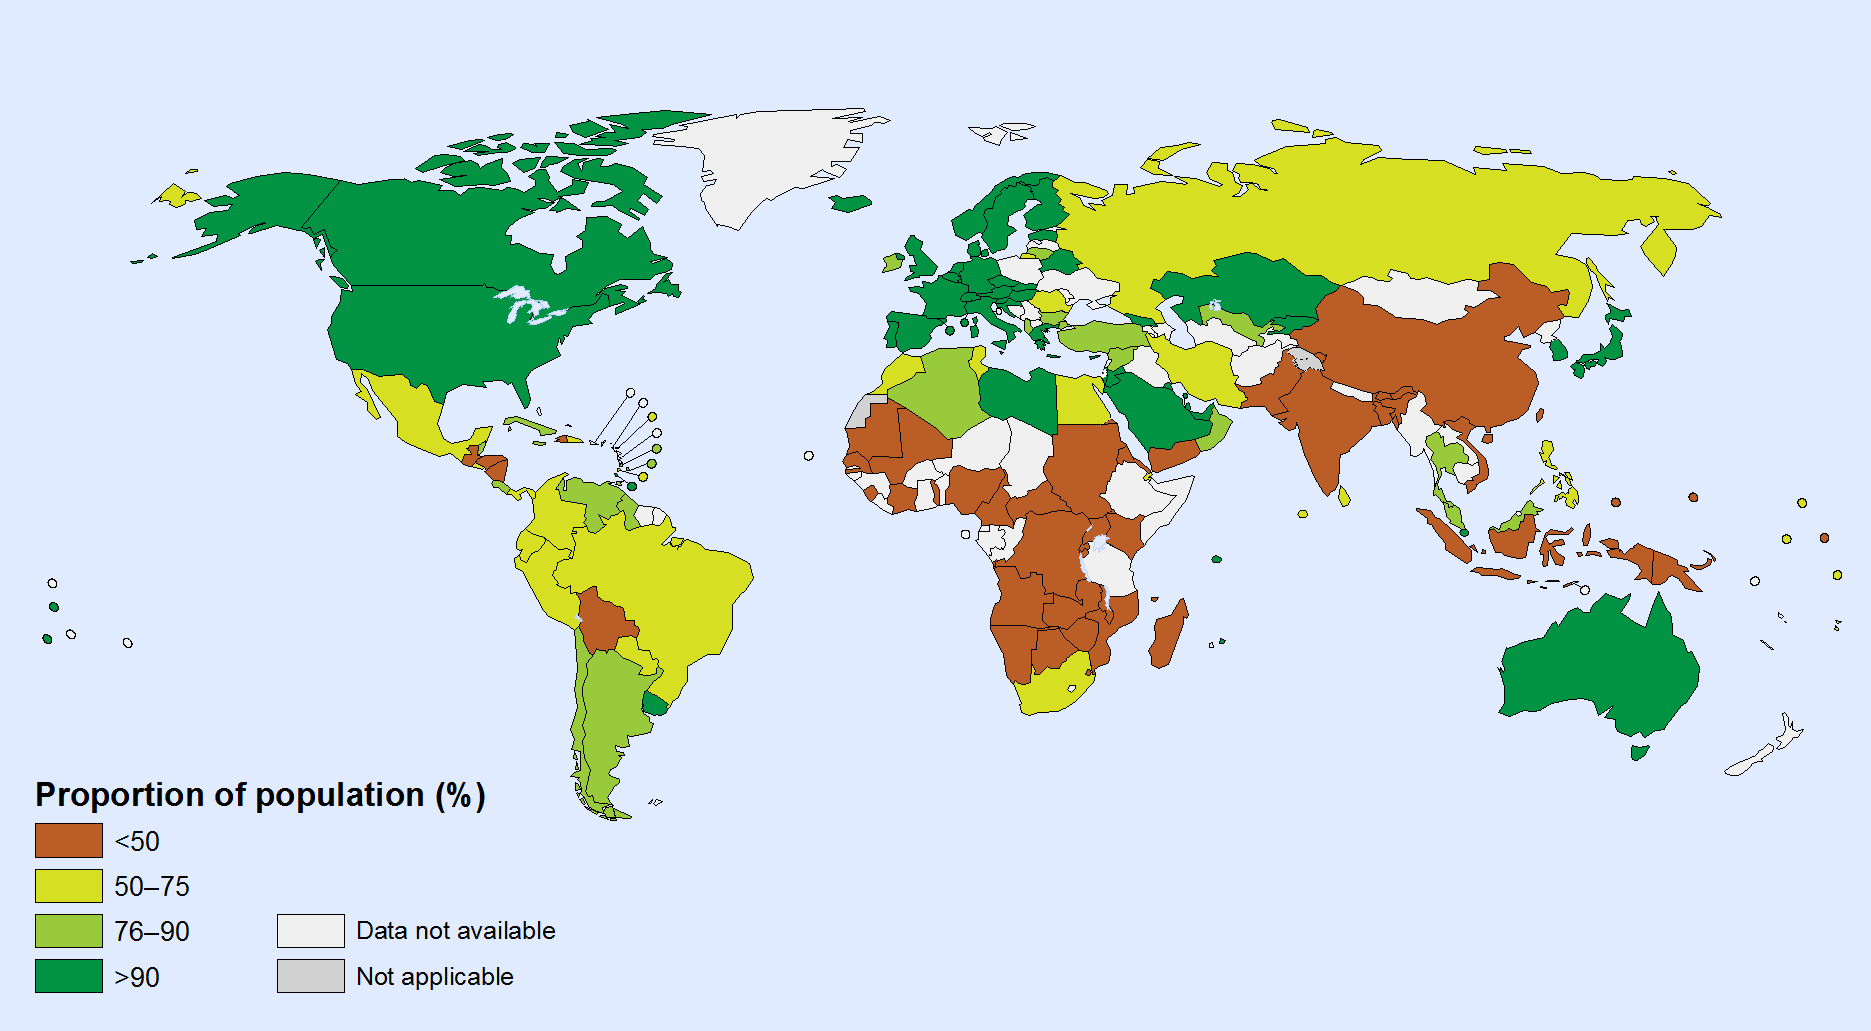
\includegraphics[width=\paperwidth]{Global_sanitation_1990}}}
\end{frame}
}

%Proportion of population using improved drinking water sources (\%), 2000
{\setbeamertemplate{frame footer}{\href{http://gamapserver.who.int/mapLibrary/Files/Maps/Global_water_2000.png}{\textcolor{gray}{http://gamapserver.who.int/mapLibrary/Files/Maps/Global\_water\_2000.png}}}
	\begin{frame}{Proportion of population using improved drinking water sources (\%), 2000}
	\makebox[\linewidth]{\parbox{\paperwidth}{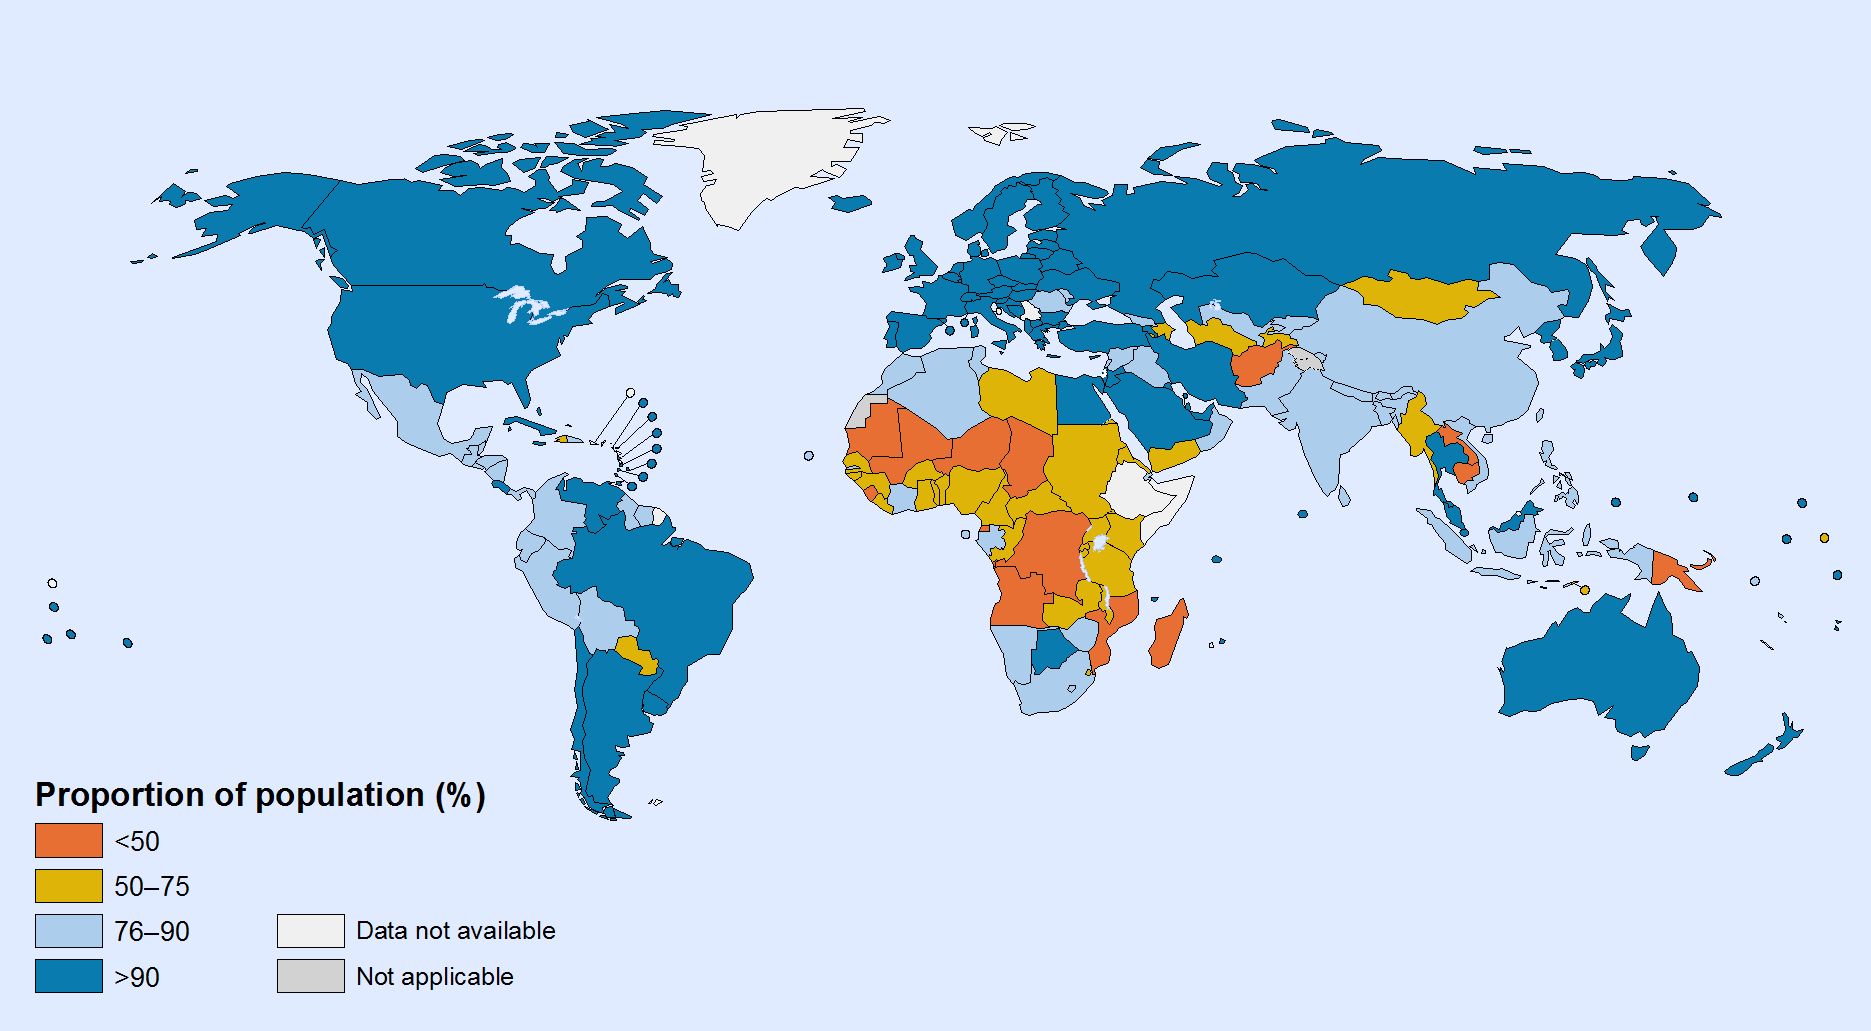
\includegraphics[width=\paperwidth]{Global_water_2000}}}
\end{frame}
}

%Proportion of population using improved sanitation facilities (\%), 2000
{\setbeamertemplate{frame footer}{\href{http://gamapserver.who.int/mapLibrary/Files/Maps/Global_sanitation_2000.png}{\textcolor{gray}{http://gamapserver.who.int/mapLibrary/Files/Maps/Global\_sanitation\_2000.png}}}
	\begin{frame}{Proportion of population using improved sanitation facilities (\%), 2000}
	\makebox[\linewidth]{\parbox{\paperwidth}{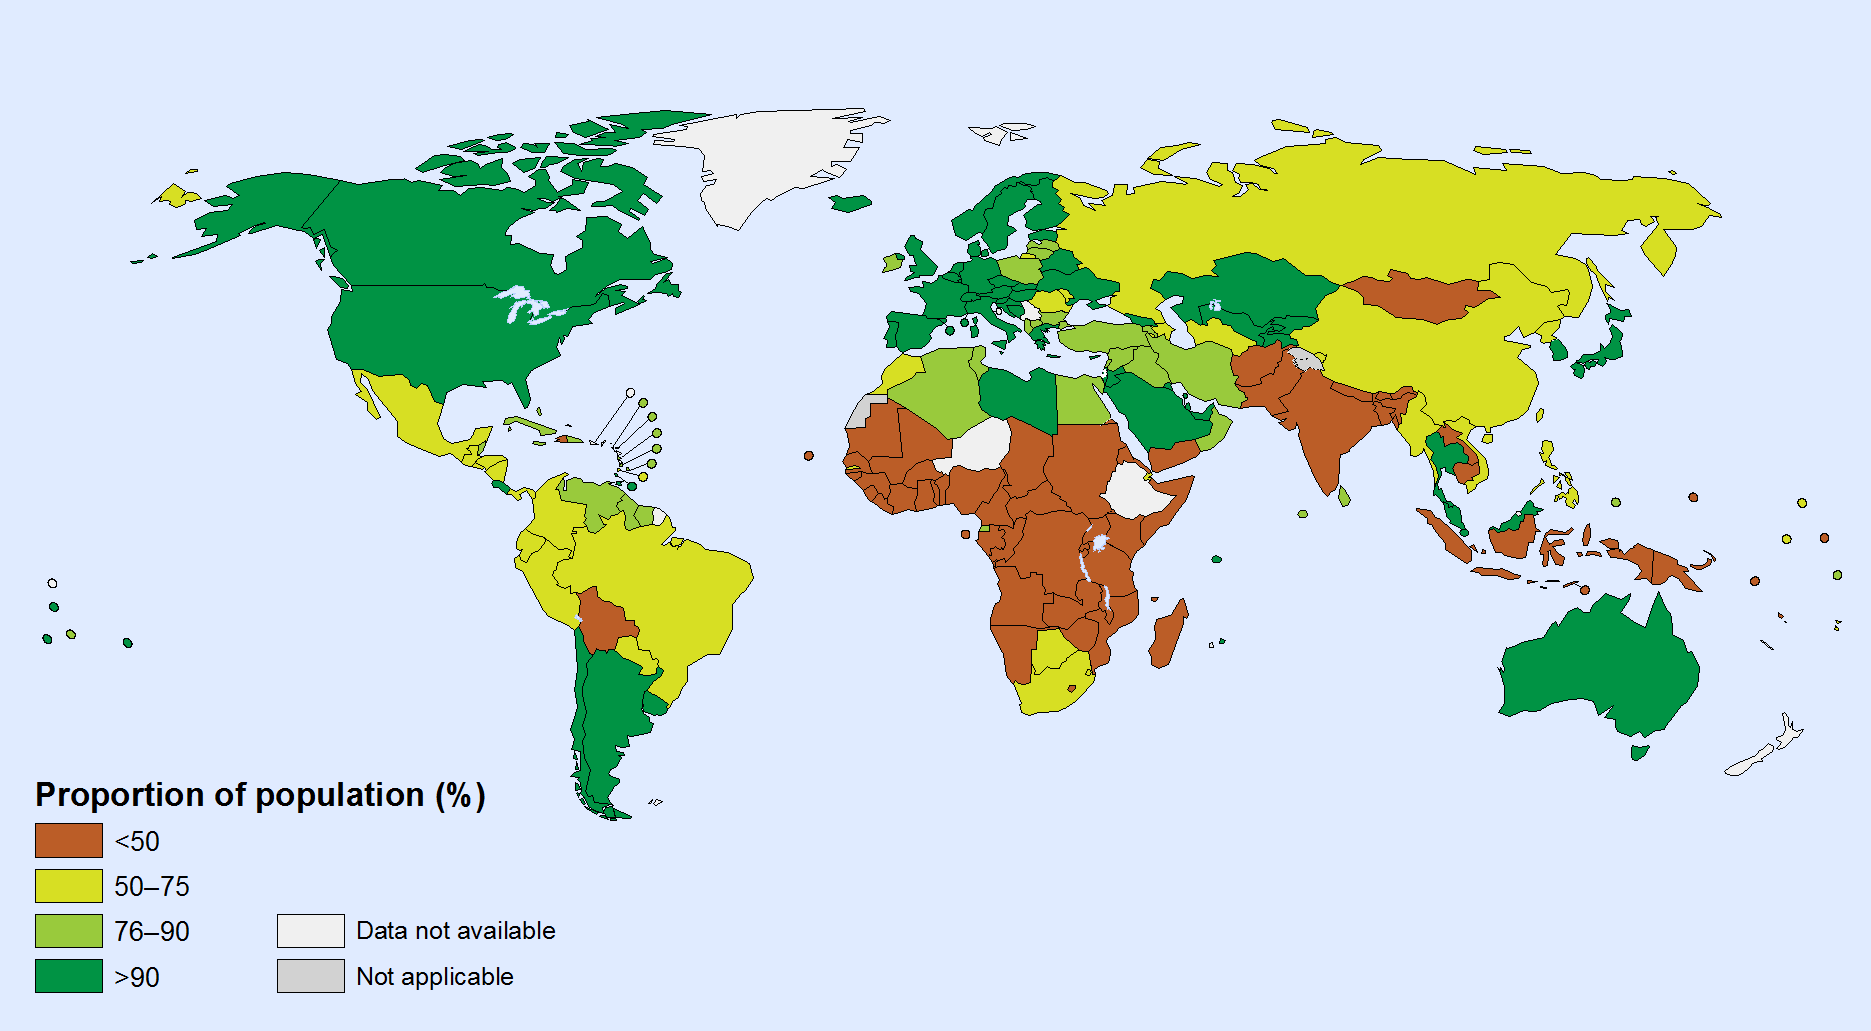
\includegraphics[width=\paperwidth]{Global_sanitation_2000}}}
\end{frame}
}

%Proportion of population using improved drinking water sources (\%), 2015
{\setbeamertemplate{frame footer}{\href{http://gamapserver.who.int/mapLibrary/Files/Maps/Global_water_2015.png}{\textcolor{gray}{http://gamapserver.who.int/mapLibrary/Files/Maps/Global\_water\_2015.png}}}
	\begin{frame}{Proportion of population using improved drinking water sources (\%), 2015}
	\makebox[\linewidth]{\parbox{\paperwidth}{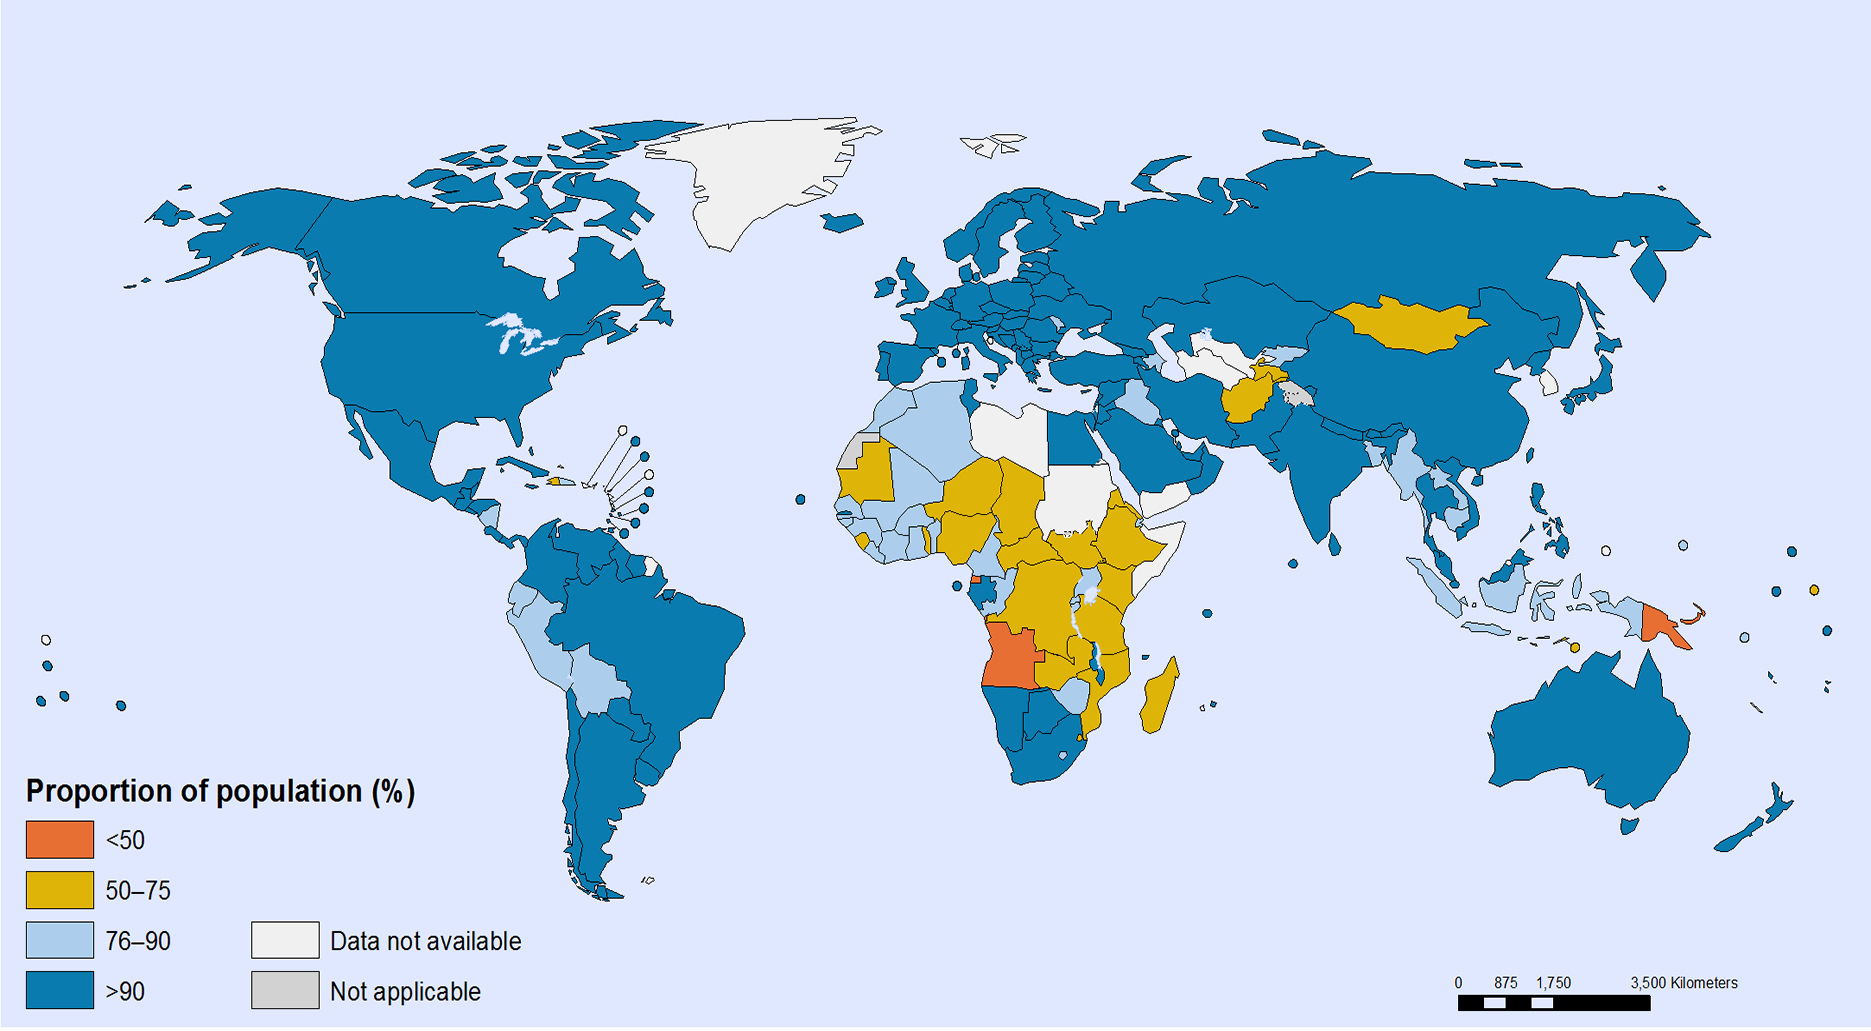
\includegraphics[width=\paperwidth]{Global_water_2015}}}
\end{frame}
}

%Proportion of population using improved sanitation facilities (\%), 2015
{\setbeamertemplate{frame footer}{\href{http://gamapserver.who.int/mapLibrary/Files/Maps/Global_sanitation_2015.png}{\textcolor{gray}{http://gamapserver.who.int/mapLibrary/Files/Maps/Global\_sanitation\_2015.png}}}
	\begin{frame}{Proportion of population using improved sanitation facilities (\%), 2015}
	\makebox[\linewidth]{\parbox{\paperwidth}{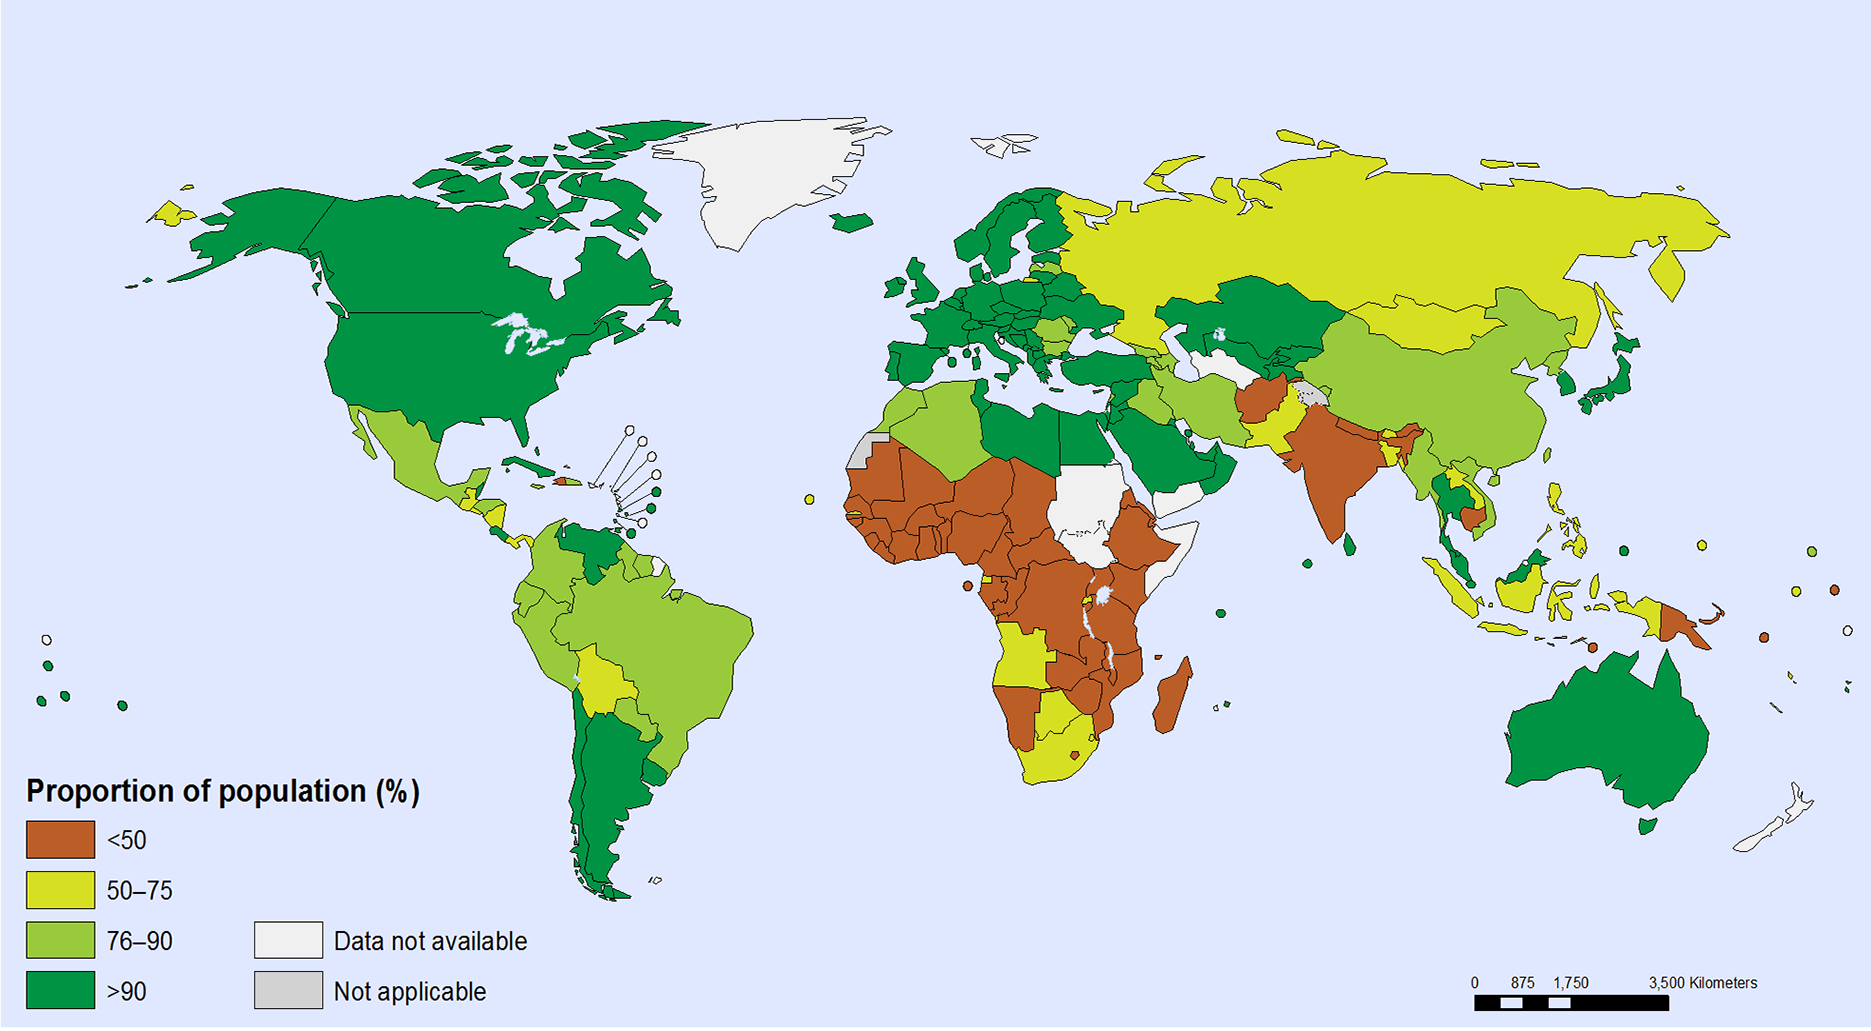
\includegraphics[width=\paperwidth]{Global_sanitation_2015}}}
\end{frame}
}

% Trophic level index of China's major lakes in 2017
{\setbeamertemplate{frame footer}{\href{http://english.mee.gov.cn/Resources/Reports/soe/SOEE2017/201808/P020180801597738742758.pdf}{\textcolor{gray}{http://english.mee.gov.cn/Resources/Reports/soe/SOEE2017/201808/P020180801597738742758.pdf}}}
	\begin{frame}{Trophic level index of China's major lakes in 2017}
	\makebox[\linewidth]{\parbox{\paperwidth}{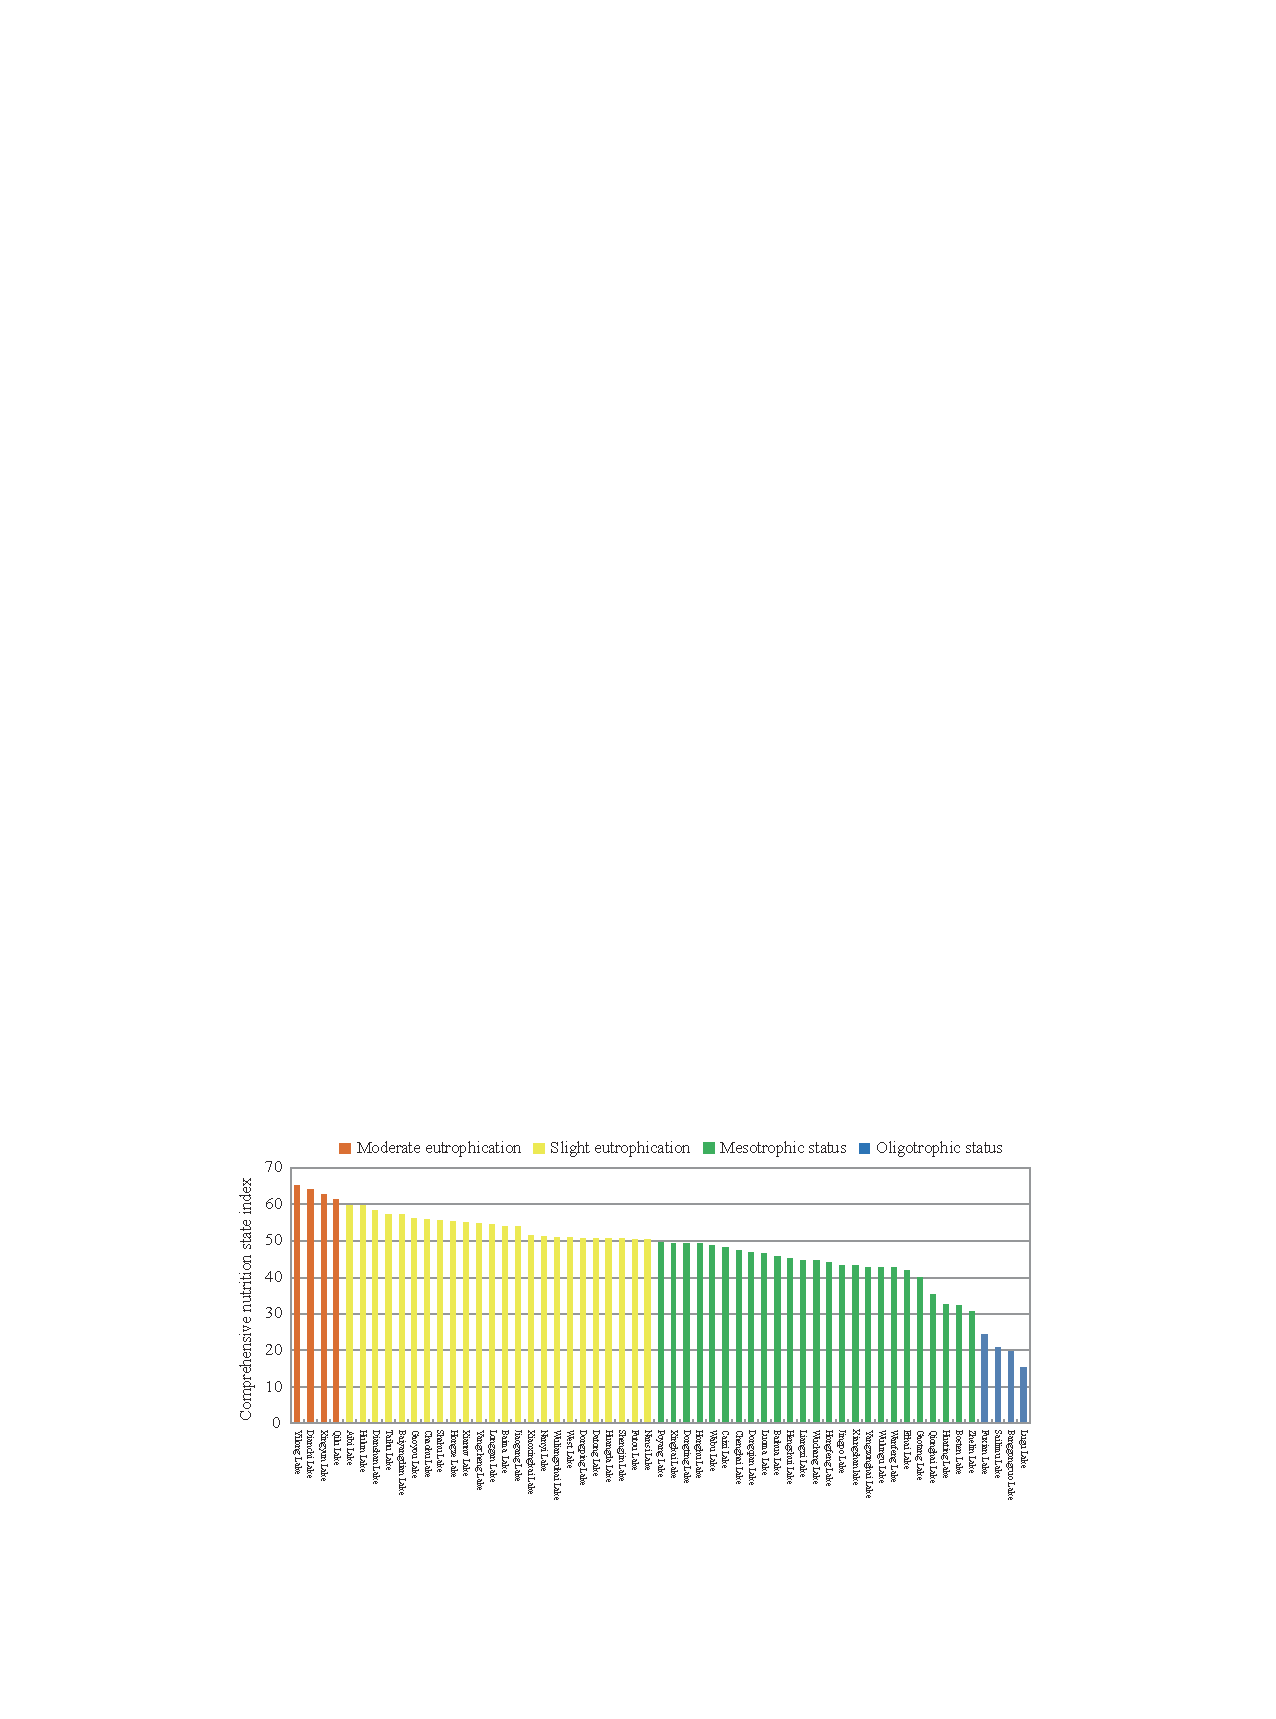
\includegraphics[width=\paperwidth]{trophic_level_index_of_major_lakes_in_china_2017.pdf}}}
\end{frame}
}

% dead zones around the word
{\setbeamertemplate{frame footer}{\href{https://eoimages.gsfc.nasa.gov/images/imagerecords/44000/44677/dead_zones_lrg.jpg}{\textcolor{gray}{https://eoimages.gsfc.nasa.gov/images/imagerecords/44000/44677/dead\_zones\_lrg.jpg}}}
	\begin{frame}{Dead zones around the world}
	\makebox[\linewidth]{\parbox{\paperwidth}{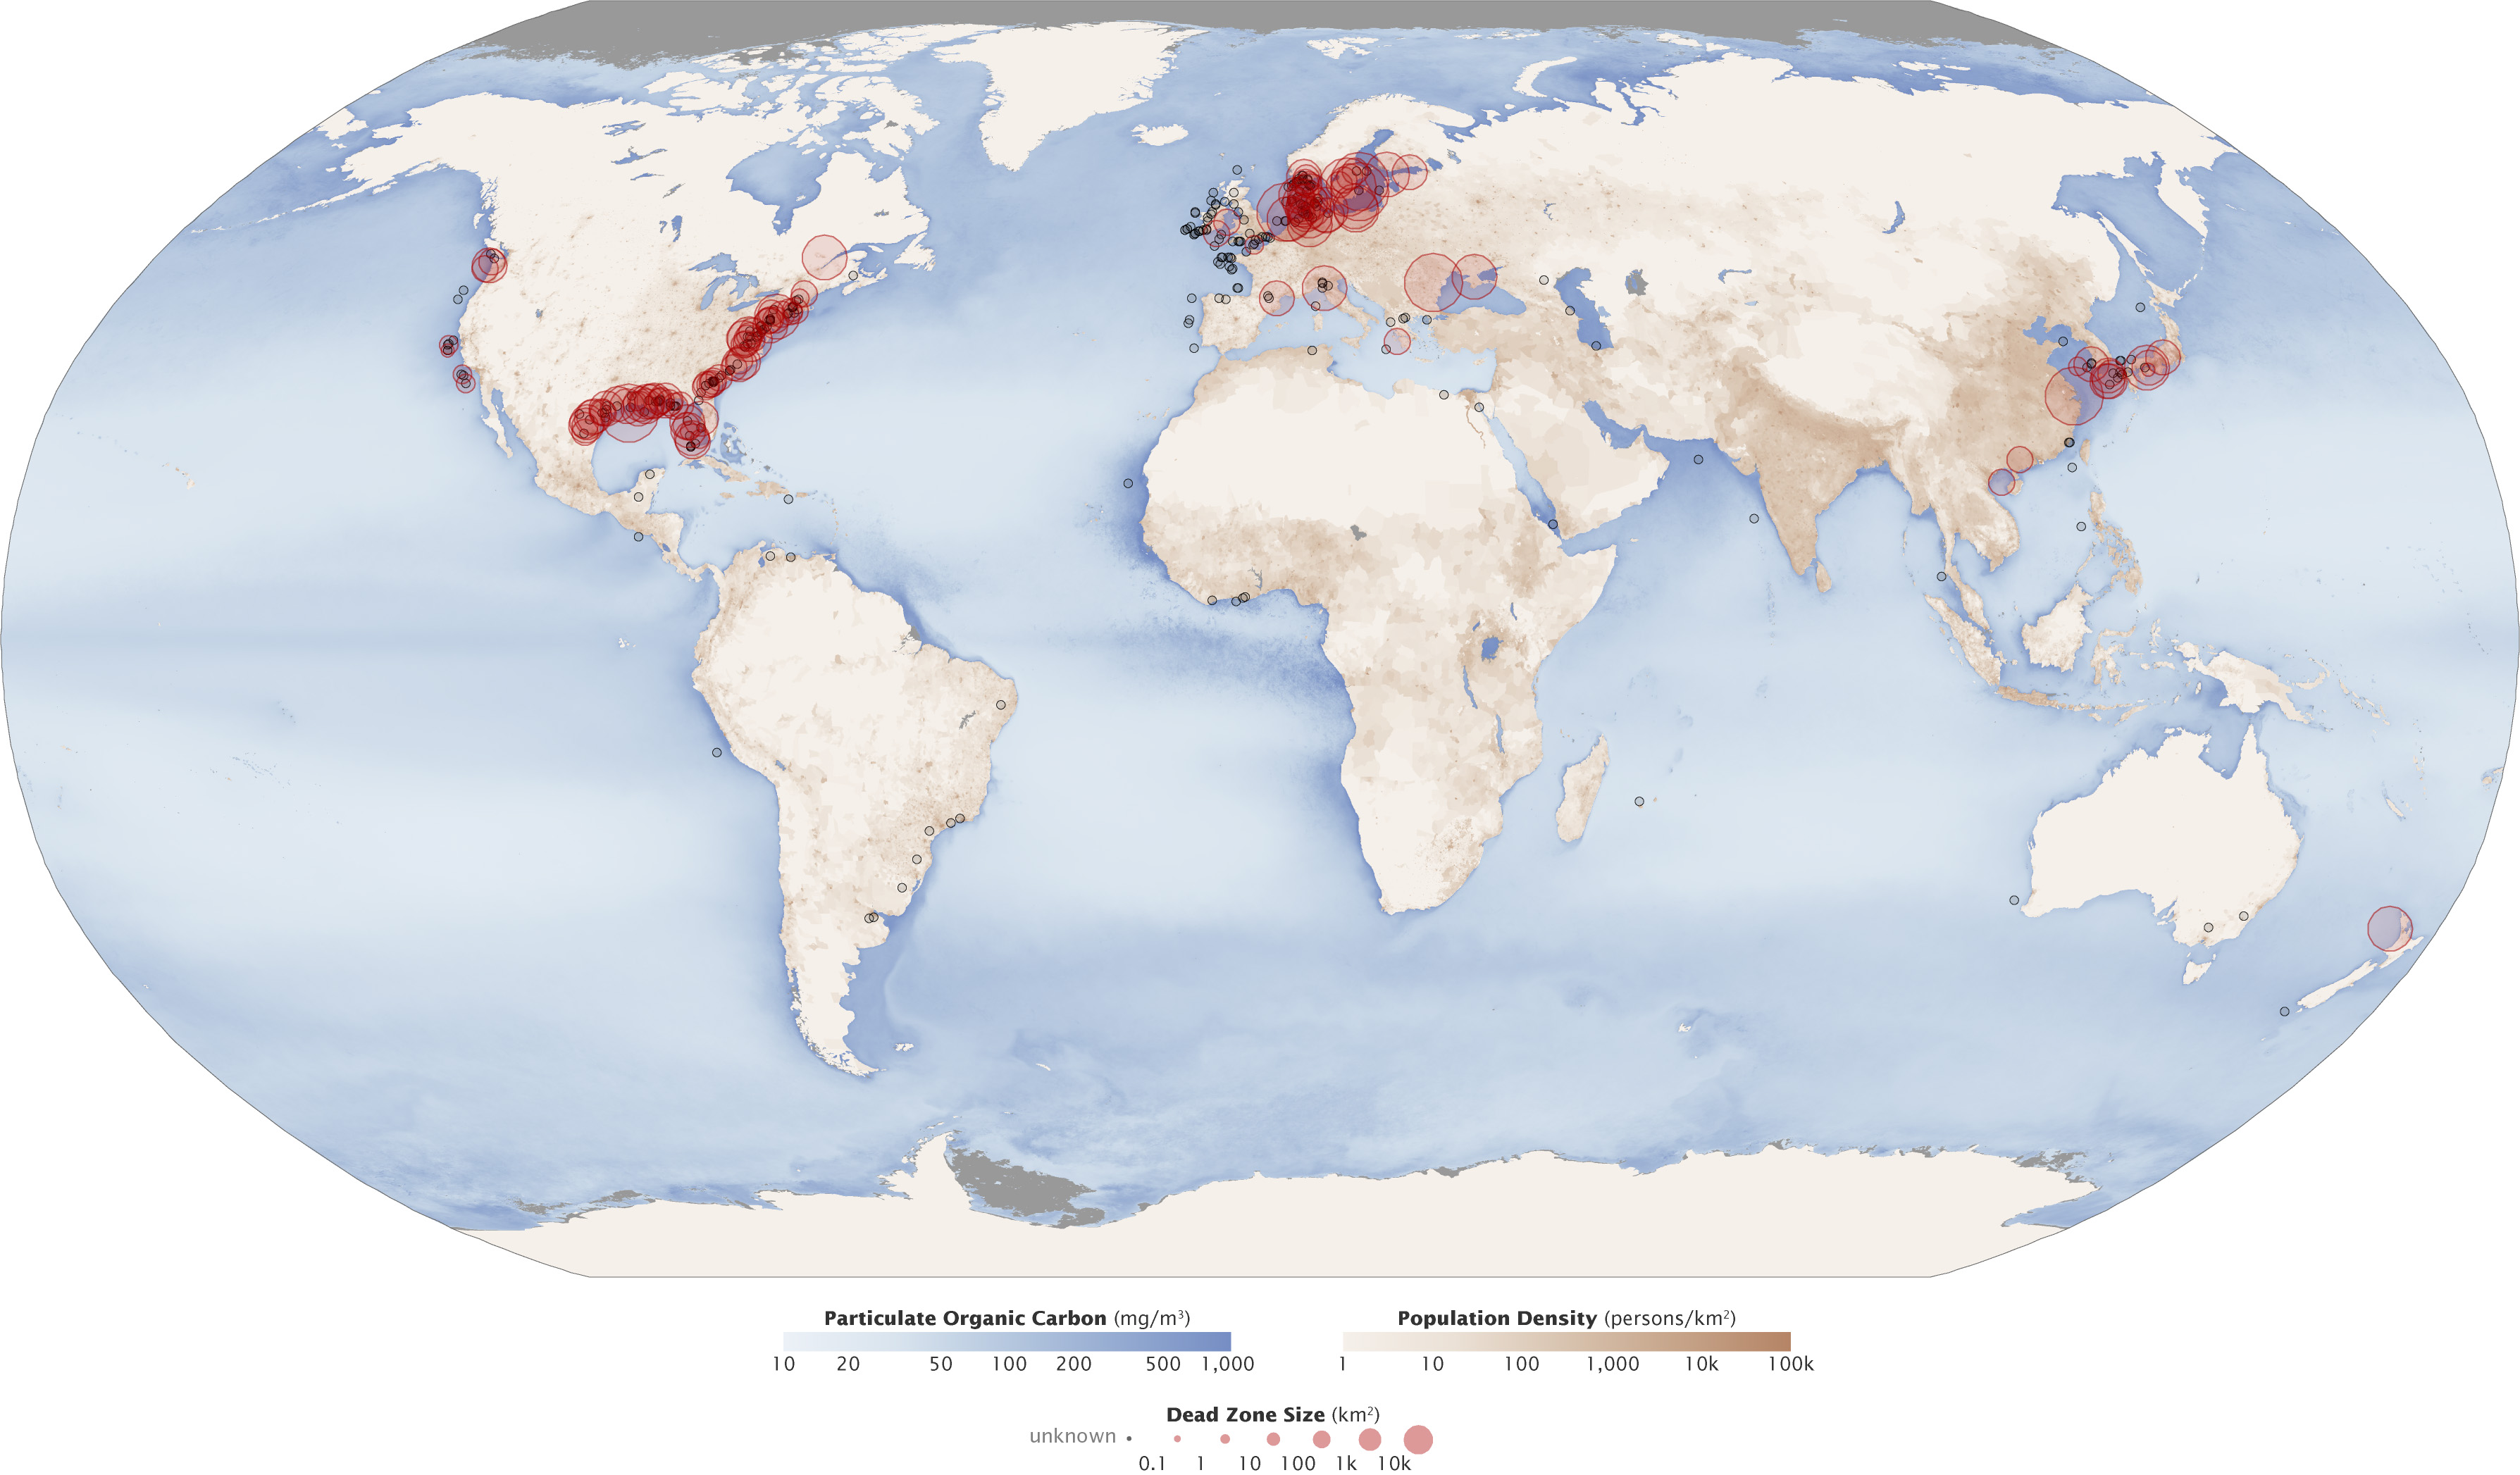
\includegraphics[width=\paperwidth]{dead_zones_lrg}}}
\end{frame}
}

% Trophic level index of China's major reservoirs in 2017
{\setbeamertemplate{frame footer}{\href{http://english.mee.gov.cn/Resources/Reports/soe/SOEE2017/201808/P020180801597738742758.pdf}{\textcolor{gray}{http://english.mee.gov.cn/Resources/Reports/soe/SOEE2017/201808/P020180801597738742758.pdf}}}
	\begin{frame}{Trophic level index of China's major reservoirs in 2017}
	\makebox[\linewidth]{\parbox{\paperwidth}{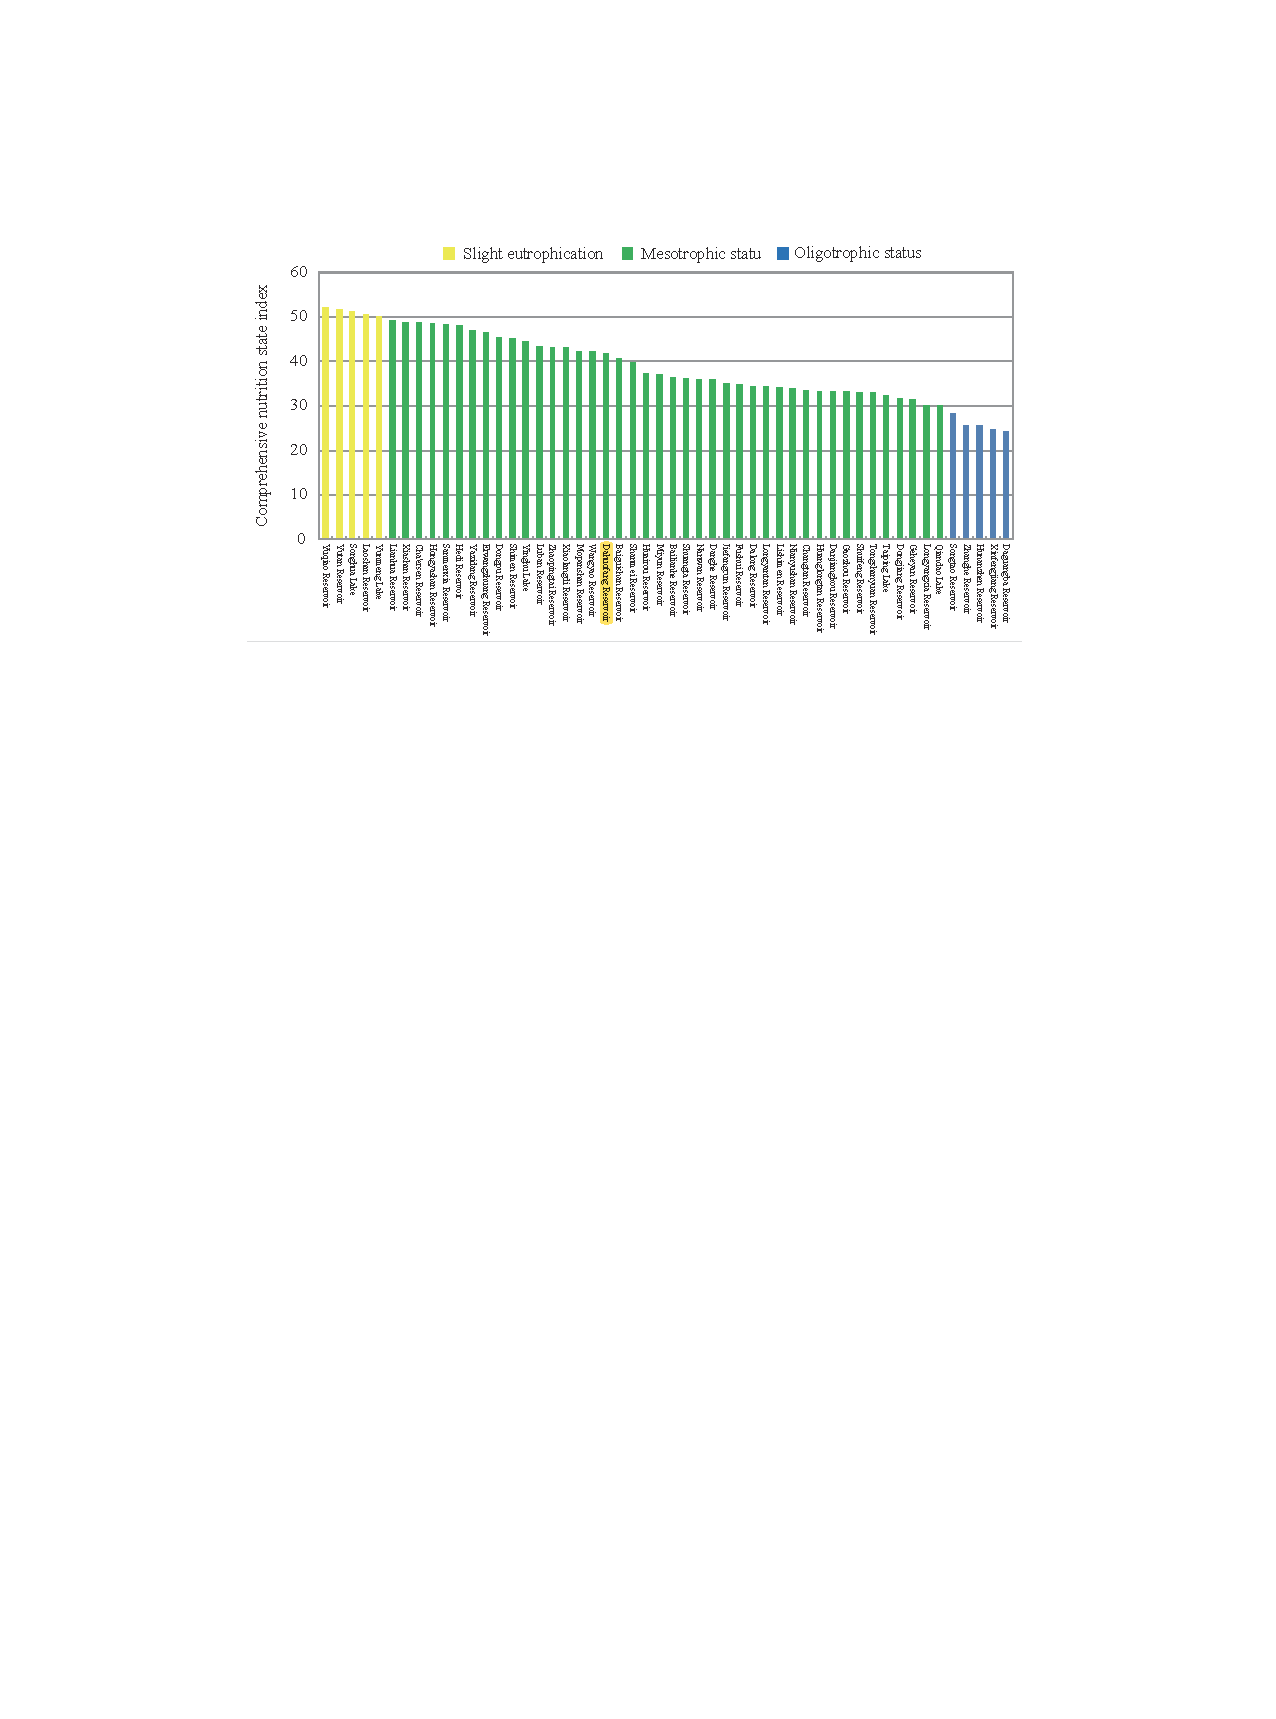
\includegraphics[width=\paperwidth]{trophic_level_index_of_major_reservoirs_in_china_2017.pdf}}}
\end{frame}
}

